\section{Vectors and the Geometry of Space}
\textit{Chapter 12: Page 794}
\subsection{3D Coordinate Systems}
Points in 3D space are represented as triples \((a,b,c)\) of real numbers. \(a\) is the \(x\) position, \(b\) is the \(y\) position, and \(c\) is the \(z\) position. 
\par
We organize 3D space by choosing an origin \(O\), and then drawing three axes for \(x\), \(y\), and \(z\) through it. \(x\) and \(y\) are typically drawn horizontally, and \(z\) is typically drawn vertically. The direction of the \(z\) axis is given by the right-hand rule. If you curl your fingers from the \(+x\) direction to the \(+y\) direction, your thumb will point in the direction of the \(+z\) direction. \par
There are three \textbf{coordinate planes} that are defined by 3D space. 
\begin{enumerate}
    \item The \(xy\) plane is the set of all vectors with a zero \(z\)-coordinate.
    \item The \(xz\) plane is the set of all vectors with a zero \(y\)-coordinate.
    \item The \(yz\) plane is the set of all vectors with a zero \(x\)-coordinate.
\end{enumerate}
These planes divide space into eight \textbf{octants}, with each octant being a unique combination of signs for the \(x\), \(y\) and \(z\) coordinates. The first octant is the set of all vectors with \(x,y,z>0\). \par
If \(P=(a,b,c)\) is a point in space, \(a\) represents the distance from the \(yz\) plane to \(P\). \(b\) represents the distance from the \(xz\) plane to \(P\), and \(c\) represents the distance from the \(xy\) plane to \(P\). We can find the \textbf{projections} of \(P\) onto any of these planes by setting the respective coordinate equal to zero:
\begin{enumerate}
    \item The projection of \(P\) onto the \(yz\) plane is given by \((0,b,c)\).
    \item The projection of \(P\) onto the \(xz\) plane is given by \((a,0,c)\).
    \item The projection of \(P\) onto the \(xy\) plane is given by \((a,b,0)\).
    \item The projection of \(P\) onto the \(x\) axis is given by \((a,0,0)\).
\end{enumerate}
The cartesian product \(\RR \times \RR \times \RR = \{(x,y,z)|x,y,z\in \RR\}\) is the set of all ordered triples. This is also denoted by \(\RR^3\). This is called the \textbf{three-dimensional rectangular coordinate system}, and has basis vectors \begin{align*}
    \ihat &= \langle 1,0,0\rangle \\
    \jhat &= \langle 0,1,0\rangle \\
    \khat &= \langle 0,0,1\rangle.
\end{align*}
An equation relating \(x\), \(y\), and \(z\) in \(\RR^3\) is called a \textit{surface} in \(\RR^3\). Some examples of surfaces are:
\begin{enumerate}
    \item \(y=3\): a plane given by the set \(\{(a,3,b)|a,b\in \RR\}\). 
    \item \(y=x\): a plane given by the set \(\{(a,a,b)|a,b,\in \RR\}\). This will look like the line \(y=x\) in \(\RR^2\), except stretched upwards infinitely in the \(z\) direction.
\end{enumerate}
The distance between two points in \(\RR^n\) given by \(P_1=(a_1, a_2, \dots a_n)\) and \(P_2=(b_1,b_2,\dots, b_n)\) is given by:
\[ |P_1P_2|=\sqrt{(b_1-a_1)^2+(b_2-a_2)^2+\dots+(b_n-a_n)^2}. \]
This can be shown with \(n-1\) repeated applications of the Pythagorean theorem. 
\begin{example}
    Find the distance between \(P(2,-1,7)\) and \(Q(1,-3,5)\). \par \textbf{Solution:}
    \begin{align*}
        |PQ|&=\sqrt{(1-2)^2+(-3+1)^2+(5-7)^2} \\
        &= \sqrt{1+4+4} = 3
    \end{align*}
\end{example}
\begin{example}
    Find an equation for a sphere with radius \(r\) and center \(C(h,k,l)\). \par 
    \textbf{Solution:} A sphere is defined as a shape where all points that lie on it are the same distance \(r\) from its center. In other words, for any point \(P(x,y,z)\) on the surface of the sphere,
    \[ \sqrt{(x-h)^2+(y-k)^2+(z-l)^2}=r \]
    or,
    \[ (x-h)^2+(y-k)^2+(z-l)^2=r^2 \]
    This result will come in handy often, and is worth remembering.
\end{example}
\begin{example}
    Show that \(x^2+y^2+z^2+4x-6y+2z+6=0\) is the equation of a sphere. Find its center and radius. \par \textbf{Solution:} First, let's rewrite our equation in a form that is more convenient to us:
    \[ (x^2+4x)+(y^2-6y)+(z^2+2z)=-6 \]
    We can complete the square to rewrite our equation:
    \[ [(x+2)^2-4]+[(y-3)^2-9]+[(z+1)^2-1]=-6. \]
    Or,
    \[ (x+2)^2+(y-3)^2+(z+1)^2=8. \]
    From this, we can see that the circle is centered at \(C(-2,3,1)\) with radius \(\sqrt 8\).
\end{example}
\begin{example}
    What region in \(\RR^3\) is represented by the following inequalities?
    \[1\leq x^2+y^2+z^2\leq 4\qquad z\leq 0\] \textbf{Soln:} The first inequality necessitates that the points are within the sphere centered at \(O\) of radius \(\sqrt 4= 2\), but outside the sphere centered at \(O\) of radius \(\sqrt 1 = 1\). The second inequality necessitates that the spheres be below or on the \(xy\) plane. Together, these describe a half-shell, with an inner radius of \(1\) and an outer radius of \(2\), that is entirely beneath or on the plane \(z=0\).
\end{example}
\subsection{Vectors}
uh something something magnitude direction. go read about it yourself
\subsection{The Dot Product}
\begin{definition}
    If \(\vec a=\< a_1, a_2, \dots, a_n\>\) and \(\vec b=\<b_1, b_2, \dots, b_n\>\), then the dot product of \(\vec a\) and \(\vec b\) is given by:
    \[\vec a \cdot \vec b = a_1b_1+a_2b_2+\dots+a_nb_n\]
\end{definition}
This gives us a useful way to "multiply" two vectors, leaving us with a scalar quantity. 
\begin{example}
    Find \begin{align*}
        \<2,4\>&\cdot \<3,-1\>, \\ \<-1, 7, 4\>&\cdot\<6,2,-\half,\>\\ \text{and }\quad (\ihat + 2\jhat - 3\khat) &\cdot (2\jhat - \khat).
    \end{align*}
     \textbf{Solution:}
     \begin{align*}
         \<2,4\>\cdot \<3,-1\>&=2\cdot 3+4\cdot (-1) = 2 \\
          \<-1, 7, 4\>\cdot\<6,2,-\half,\> &= -1 \cdot 6 + 7\cdot 2 + 4 \cdot -\half \\
          &= -6+14-2 = 6 \\
          (\ihat + 2\jhat - 3\khat) \cdot (2\jhat - \khat) &= 1\cdot 0 + 2\cdot 2 +(-3)\cdot (-1) \\
          &=4+3 = 7
     \end{align*}
\end{example}
\begin{theorem}[Properties of the Dot Product]
    If \(\vec a, \vec b, \vec c \in V\), where \(V\) is a vector space, and \(k\in \RR\):
    \begin{enumerate}
        \item \(\vec a \cdot \vec a = |\vec a|^2\) 
        \item \(\vec a \cdot (\vec b + \vec c) = \vec a\cdot \vec b + \vec a \cdot \vec c\)
        \item \(\vec a \cdot \vec 0 = 0\)
        \item \(\vec a \cdot \vec b = \vec b \cdot \vec a\)
        \item \((k\vec a)\cdot b=k(\vec a\cdot \vec b)=a\cdot (k\vec b)\)
    \end{enumerate}
\end{theorem}
These can all be proven quite easily:
\begin{proof}
    Let \(\vec a = \<a_1, a_2, \dots, a_n\>\), \(\vec b = \<b_1, b_2, \dots, b_n\>\), \(\vec c = \<c_1, c_2, \dots, c_n\>\), and let \(k\in \RR\). Then,
    \begin{align*}
        \vec a \cdot \vec a &= a_1a_1+a_2a_2+\dots+a_na_n=a_1^2+a_2^2+\dots+a_n^2\\&=|\vec a|^2\text{ (Property 1).} \\
        \vec a \cdot (\vec b + \vec c) &= a_1(b_1+c_1)+a_2(b_2+c_2)+\dots+a_n(b_n+c_n) \\
        &= a_1b_1+a_1c_1+a_2b_2+a_2c_2+\dots+a_nb_n+a_nc_n \\
        &= \vec a\cdot \vec b + \vec a \cdot \vec c \text{ (Property 2).} \\
        \vec a \cdot \vec 0 &= 0a_1+0a_2+\dots+0a_n \\ 
        &= 0\text{ (Property 3).} \\
        \vec a \cdot \vec b &= a_1b_1+a_2b_2+\dots+a_nb_n \\
        &= b_1a_1 + b_2a_2+\dots+b_na_n \\
        &= \vec b \cdot \vec a \text{ (Property 4).} \\
        (k\vec a)\cdot \vec b &= (ka_1)b_1+(ka_2)b_2+\dots+(ka_n)b_n \\
        &= k(a_1b_1+a_2b_2+\dots+a_nb_n) \\
        &= k(\vec a \cdot \vec b) \\
        (k\vec a)\cdot \vec b &= (ka_1)b_1+(ka_2)b_2+\dots+(ka_n)b_n \\
        &= a_1(kb_1)+a_2(kb_2)+\dots+a_n(kb_n) \\
        &= \vec a \cdot (k\vec b) \text{ (Property 5).}
    \end{align*}
\end{proof}
There is also a geometric interpretation of the dot product,
\begin{theorem}
    If \(\vec a, \vec b\in \RR^n\) and \(\theta\) is the angle between them, then
    \[\vec a\cdot \vec b = |\vec a|\,|\vec b|\cos\theta\]
\end{theorem}
\begin{proof}
    Create a triangle with vertices \(OAB\). Define \(\vec a = \overrightarrow{OA}\) and \(\vec b = \overrightarrow{OB}\). Then, by the law of cosines,
    \begin{align*}
        |\overrightarrow{AB}|^2 &= |\overrightarrow{OA}|^2+|\overrightarrow{OB}|^2-2|\overrightarrow{OA}|\,|\overrightarrow{OB}|\cos\theta \\
        &= |\vec a|^2 + |\vec b|^2 - 2|\vec a|\,|\vec b|\cos \theta
    \end{align*}
    We can also note that \(\overrightarrow{AB}=\vec a - \vec b\). Then,
    \begin{align*}
        |\vec a - \vec b|^2 &= |\vec a|^2 + |\vec b|^2 - 2|\vec a|\,|\vec b|\cos \theta \\
        |\vec a|^2 -2(\vec a \cdot \vec b)+|\vec b|^2 &= |\vec a|^2 + |\vec b|^2 - 2|\vec a|\,|\vec b|\cos \theta \\
        -2(\vec a \cdot \vec b) &= -2|\vec a|\,|\vec b|\cos \theta \\
        \vec a\cdot \vec b &= |\vec a|\,|\vec b|\cos\theta
    \end{align*}
\end{proof}
Using this, we can come to a quite significant conclusion:
\begin{corollary}
    If \(\theta\) is the angle between two nonzero vectors \(\vec a\) and \(\vec b\), then
    \[\cos \theta = \frac{\vec a \cdot \vec b}{|\vec a|\,|\vec b|}\]
\end{corollary}
This can be used to find the angle between two vectors, given their components (or their magnitudes and dot products).
\begin{example}
    Find the angle between \(\vec a = \<2, 2, -1\>\) and \(\vec b = \<5, -3, 2\>\). \par \textbf{Solution:} First, determine that \[|\vec a| = \sqrt{2^2+2^2+(-1)^2}=3\]
    and \[|\vec b| = \sqrt{5^2+(-3^2)+2^2}=\sqrt{38}.\]
    Then, find that \[\vec a \cdot \vec b = 2\cdot 5 - 3\cdot 2-2\cdot 1 = 2.\] Then, calculate that \[\theta = \cos^{-1}\left(\frac{2}{3\sqrt {38}}\right)\approx 1.46 \approx 0.46\pi\]
\end{example}
Theorem 1.3.4 also leads to an interesting conclusion about orthogonal vectors. \begin{theorem}
    Two vectors \(\vec a, \vec b \in \RR^n\) are orthogonal if and only if \[\vec a \cdot \vec b = 0.\]
\end{theorem}\begin{proof}
    Let \(\vec a, \vec b \in \RR^n\), and let \(\theta\) be the angle between \(\vec a\) and \(\vec b\). \par
    By the definition of orthogonal, the angle between \(\vec a\) and \(\vec b\) must be \(\theta = \pi/2\). Then, by the definition of the dot product,
    \[\vec a \cdot \vec b = |\vec a|\,|\vec b|\cos\theta = |\vec a|\,|\vec b|\cos\frac{\pi}{2}=0.\]
\end{proof}
Further, since \(\cos\theta > 0\) for \(\theta \in (0, \pi/2)\), \(\vec a\cdot \vec b>0\) implies that the angle between them is acute. Similarly, since \(\cos\theta < 0\) for \(\theta \in (\pi/2, \pi)\), \(\vec a \cdot \vec b<0\) implies that the angle between them is obtuse. \par
If \(\vec a\) and \(\vec b\) are pointing in the same direction, the angle between them is \(0\) and \(\vec a\cdot\vec b = |\vec a|\,|\vec b|\). \par
Likewise, if \(\vec a\) and \(\vec b\) are pointing in opposite directions, the angle between them is \(\pi\) radians and \(\vec a\cdot\vec b = -|\vec a|\,|\vec b|\).
\subsubsection{Direction Angles and Direction Cosines}
The \textit{direction angles} of a nonzero vector \(\vec a \in \RR^3\) are the angles \(\alpha\), \(\beta\), and \(\gamma\) that \(\vec a\) makes with the positive x-, y-, and z- axes. \par
The cosines of these direction angles, \(\cos \alpha\), \(\cos\beta\), and \(\cos\gamma\) are called the \textit{direction cosines} of \(\vec a\). By Corollary 1.3.5, we can obtain formulas for each of these:
\begin{align*}
    \cos \alpha = \frac{\vec a \cdot  \ihat}{|\vec a|} &= \frac{a_1}{|\vec a|} \\
    \cos \beta = \frac{\vec a \cdot \jhat}{|\vec a|} &= \frac{a_2}{|\vec a|} \\
    \cos \gamma = \frac{\vec a \cdot \khat}{|\vec a|} &= \frac{a_3}{|\vec a|}
\end{align*}
Another consequence of this is that
\[\cos^2\alpha + \cos^2\beta + \cos^2\gamma = \frac{1}{|\vec a|^2}(a_1^2+a_2^2+a_3^2) = 1\]
\begin{example}
    Find the direction angles of \(\vec a = \<1,2,3\>\). \par
    \textbf{Solution: }
    First, find \[|\vec a| = \sqrt{1^2+2^2+3^2}=\sqrt{14}\]
    then,
    \[\alpha = \cos^{-1} \frac{1}{\sqrt{14}} \quad \beta = \cos^{-1}\frac{2}{\sqrt{14}} \quad \gamma = \cos^{-1}\frac{3}{\sqrt{14}}\]
\end{example}
\subsection{Projections}
With dot products, we can \textit{project} two vectors onto each other. Consider two vectors \(\vec a, \vec b \in \RR^n\). We can denote the \textit{vector projection} of \(\vec b\) onto \(\vec a\) with \(\proj{\vec a}{\vec b}\). \par 
Similarly, we can define the \textit{scalar projection} of \(\vec b\) onto \(\vec a\) (also called the \textit{component of \(\vec b\) along \(\vec a\)}) as the magnitude of the vector projection, or:
\[\comp{\vec a}{\vec b}=|\proj{\vec a}{\vec b}|\]
This can also be found with:
\[\comp{\vec a}{\vec b} = \frac{\vec a\cdot \vec b}{|\vec a|} = |\vec b|\cos\theta \]
Alternatively,
\[\comp{\vec a}{\vec b}= \frac{\vec a}{|\vec a|}\cdot \vec b\]
Then, the vector projection is:
\begin{align*}
    \proj{\vec a}{\vec b}&=\comp{\vec a}{(\vec b)}\frac{\vec a}{|\vec a|} \\ &= \left(\frac{\vec a\cdot \vec b}{|\vec a|}\right) \frac{\vec a}{|\vec a|} \\
    &= \frac{\vec a \cdot \vec b}{|\vec a|^2}\vec a
\end{align*}
\begin{example}
    Find the scalar and vector projection of \(\vec b = \<1,1,2\>\) onto \(\vec a =\<-2, 3, 1\>\). \par
    \textbf{Solution: }First, 
    \[\comp{\vec a}{\vec b} = \frac{\vec a\cdot \vec b}{|\vec a|} = \frac{1\cdot (-2) + 1\cdot 3 + 2\cdot 1}{\sqrt{(-2)^2+3^2+1^2}} = \frac{3}{\sqrt{14}}\]
\end{example}
Then, \[\proj{\vec a}{\vec b} = \hat{a}\comp{\vec a}{\vec b} = \frac{3}{\sqrt{14}}\<\frac{-2}{\sqrt{14}}, \frac{3}{\sqrt{14}},\frac{1}{\sqrt{14}}\> = \<-\frac{3}{7}, \frac{9}{14}, \frac{3}{14}\>\]
\subsection{The Cross Product}
The cross product is a special operation defined only for three-dimensional vectors. Specifically,
\begin{definition}
    If \(\vec a = \< a_1, a_2, a_3\>\) and \(\vec b = \<b_1, b_2, b_3\>\), then the cross product between \(\vec a\) and \(\vec b\) is:
    \[\vec a \times \vec b = \<a_2b_3 - a_3b_2, a_3b_1-a_1b_3, a_1b_2-a_2b_1\>\]
\end{definition}
This is easily remembered as the determinant of the matrix:
\[ \vec a \times \vec b = \begin{vmatrix}
    \ihat & \jhat & \khat \\
    a_1 & a_2 & a_3 \\
    b_1 & b_2 & b_3
\end{vmatrix} \]
\begin{example}
    Show that \(\vec a \times \vec a = \vec 0\) for any \(\vec a \in \RR^3\). \par 
    \textbf{Solution: } Let \(\vec a = \<a_1, a_2, a_3\>\). Then, \[\vec a \times \vec a = \<a_2a_3-a_3a_2, a_3a_1-a_1a_3, a_1a_2-a_2a_1\> = \<0,0,0\>=\vec 0\]
\end{example}
Another critical property of the cross product,
\begin{theorem}
    For any \(\vec a, \vec b \in \RR^3\), \(\vec a \times \vec b\) is orthogonal to both \(\vec a\) and \(\vec b\).
\end{theorem}
\begin{proof}
    First, \(\vec a \times \vec b\) is orthogonal to \(\vec a\):
    \begin{align*}
        (\vec a \times \vec b) \cdot \vec a &= a_1(a_2b_3-a_3b_2) - a_2(a_1b_3-a_3b_1) + a_3(a_1b_2 - a_2b_1) \\
        &= a_1a_2b_3 - a_1a_3b_2 - a_1a_2b_3 + a_2a_3b_1 + a_1a_3b_2 - a_2a_3b_1 \\
        &= (a_1a_2b_3 - a_1a_2b_3) + (a_1a_3b_2 - a_1a_3b_2) + (a_2a_3b_1 - a_2a_3b_1) \\
        &= 0
    \end{align*}
    Then, \(\vec a \times \vec b\) is orthogonal to \(\vec b\):    \begin{align*}
        (\vec a \times \vec b) \cdot \vec b &= b_1(a_2b_3-a_3b_2) - b_2(a_1b_3-a_3b_1) + b_3(a_1b_2 - a_2b_1) \\
        &= a_2b_1b_3 - a_3a_1b_2 - a_1b_2b_3 + a_3b_1b_2 + a_1b_2b_3 - a_2b_1b_3 \\
        &= (a_2b_1b_3 - a_2b_1b_3) + (a_3a_1b_2 - a_3a_1b_2) + (a_1b_2b_3 - a_1b_2b_3) \\
        &= 0
    \end{align*}
\end{proof}
This means that if \(\vec a\) and \(\vec b\) are represented as directed line segments coming from the same initial point, then \(\vec a \times \vec b\) point in a direction perpendicular to the plane through \(\vec a\) and \(\vec b\). The direction of this is determined by the \textit{right-hand rule}: If the fingers of your right hand curl in the direction of rotation from \(\vec a\) to \(\vec b\), then your thumb points in the direction of \(\vec a\times \vec b\).
\par 
Another important property of the cross product:
\begin{theorem}
    Let \(\vec a, \vec b\in \RR^n\) be nonzero vectors, and let \(\theta\) be the angle between them. Then, \[|\vec a\times \vec b| = |\vec a|\,|\vec b|\,\sin\theta\]
\end{theorem}
\begin{proof}
    \begin{align*}
        |\vec a \times \vec b|^2 &= (a_2b_3-a_3b_2)^2+(a_3b_1-a_1b_3)^2+(a_1b_2-a_2b_1)^2 \\
        &= a_2^2b_3^2-2a_2b_3a_3b_2+a_3^2b_2^2 + a_3^2b_1^2-2a_3b_1a_1b_3+a_1^2b_3^2 \\ 
        &+ a_1^2b_2^2 - 2a_1b_2a_2b_1 + a_2^2b_1^2 \\
        &= (a_1^2+a_2^2+a_3^2)(b_1^2+b_2^2+b_3^2)-(a_1b_1+a_2b_2+a_3b_3)^2 \\
        &= |\vec a|^2|\vec b|^2 - (\vec a \cdot \vec b)^2 \\
        &= |\vec a|^2|\vec b|^2 - |\vec a|^2|\vec b|^2\cos^2\theta \\
        &= |\vec a|^2|\vec b|^2(1-\cos^2\theta) \\
        &= |\vec a|^2|\vec b|^2\sin^2\theta \\
        |\vec a \times \vec b| &= |\vec a|\,|\vec b|\sin\theta
    \end{align*}
\end{proof}
Additionally,
\begin{corollary}
    Two nonzero vectors \(\vec a, \vec b \in \RR^3\) are parallel or antiparallel if and only if \[\vec a \times \vec b = \vec 0\]
\end{corollary}
This easily follows from the magnitude definition of the cross product, where \(\sin\theta = 0\) if \(\theta = 0\) or \(\theta = \pi\). \par
There is also a geometric interpretation of the cross product: if \(\vec a, \vec b\in \RR^3\), then \(|\vec a \times \vec b|\) is the area of the parallelogram determined by \(\vec a\) and \(\vec b\) (see the below image).
\picture{0.4\textwidth}{parallelogram.png}
\begin{example}
    Find a vector perpendicular to the plane that passes through the points \(P(1,4,6)\), \(Q(-2,5,-1)\), and \(R(1,-1,1)\). \par \textbf{Solution:} First, consider the vectors \(\overrightarrow{PQ}=\<-3, 1, -7\>\) and \(\overrightarrow{PR}=\<0,-5,-5\>\). Then, if \(\hat N\) is the unit normal vector to the plane, 
    \[ \hat N = \frac{\overrightarrow{PQ}\times\overrightarrow{PR}}{|\overrightarrow{PQ}\times\overrightarrow{PR}|}=\frac{\<-40, -15, 15\>}{\sqrt{40^2+15^2+15^2}}=\frac{1}{\sqrt{82}}\<-8, -3, 3\> \] 
    Then, for any \(a\in\RR\), \(a\hat N\) is perpendicular to the plane.
\end{example}
\begin{example}
    Find the area of the triangle with vertices \(P, Q, R\) (from the previous example). \par 
    \textbf{Solution:} We've already determined that \[|\overrightarrow{PQ}\times\overrightarrow{PR}|=5\sqrt{82}\] in the previous part. We can interpret this as the area of the parallelogram formed by \(\overrightarrow{PQ}\) and \(\overrightarrow{PR}\). The triangle will have half the area of the parallelogram, or \(A=\frac{5}{2}\sqrt{82}\).
\end{example}
Some other important properties of the cross product,
\begin{theorem}
    If \(\vec a, \vec b, \vec c\in \RR^3\) and \(x\in\RR\),
    \begin{enumerate}
        \item \(\vec a \times \vec b = -(\vec b\times \vec a)\). 
        \item \((x\vec a)\times \vec b = x(\vec a \times \vec b)= \vec a \times (x\vec b)\).
        \item \(\vec a \times (\vec b + \vec c) = \vec a \times \vec b + \vec a \times \vec c\).
        \item \((\vec a + \vec b)\times \vec c = \vec a \times \vec c + \vec b \times \vec c\).
        \item \(\vec a \cdot (\vec b \times \vec c) = (\vec a \times \vec b)\cdot \vec c\).
        \item \(\vec a \times (\vec b \times \vec c) = (\vec a \cdot \vec c)\vec b - (\vec a \cdot \vec b)\vec c\).
    \end{enumerate}
\end{theorem}
These properties can be shown relatively easily (although it is a bit of annoying algebra). \par
One of these properties, Property 5, is especially important. It is known as the \textbf{scalar triple product} of \(\vec a\), \(\vec b\), and \(\vec c\). If \(\vec a = \<a_1,a_2,a_3\>\), and \(\vec b \times \vec c =\<d_1, d_2,d_3\>\), we can rewrite:
\[\vec a \cdot (\vec b \times \vec c) = a_1(d_1)+a_2(d_2)+a_3(d_3)\]
Which is also equal to the determinant
\[ \vec a \cdot (\vec b \times \vec c)=\begin{vmatrix}
    a_1 & a_2 & a_3 \\
    b_1 & b_2 & b_3 \\
    c_1 & c_2 & c_3
\end{vmatrix}, \]
since \( d_1=\begin{vmatrix}
    b_2 & b_3 \\
    c_2 & c_3
\end{vmatrix} \), \(d_2 = \begin{vmatrix}
    b_1 & b_3 \\
    c_1 & c_3
\end{vmatrix},\) and \(d_3 = \begin{vmatrix}
    b_1 & b_2 \\
    c_1 & c_2
\end{vmatrix}\). \par
There is also a geometric interpretation of the scalar triple product. Consider the parallelepiped formed by \(\vec a, \vec b\), and \(\vec c\) (below).
\picture{0.4\textwidth}{parallelepiped.png}
The area of the base of the shape is given by \(A=|\vec b\times \vec c|\). If \(\theta\) is the angle between \(\vec a\) and \(\vec b\times \vec c\), then the height is given by \(h=|\vec a|\, |\cos\theta|\) (note that we must use \(|\cos\theta|\) instead of \(\cos \theta\) in case \(\theta>\pi/2\)). Then, the total volume,
\[V=Ah=|\vec a|\,|\cos\theta|\,|\vec b \times \vec c| = |\vec a \cdot (\vec b \times \vec c)|\]
which we can recognize as the scalar triple product between \(\vec a\), \(\vec b\), and \(\vec c\). \par 
Another application of this formula is when the volume of the paralellepiped is \(0\), which we can recognize happens when \(\vec a\), \(\vec b\), and \(\vec c\) exist in the same plane. This is referred to as them being \textbf{coplanar}.
\begin{example}
    Use the scalar triple product to show that the vectors \(\vec a = \<1,4,-7\>\), \(\vec b =\<2, -1, 4\>\), and \(\vec c = \<0, -9, 18\>\) are coplanar. \par
    \textbf{Solution:} 
    \[ \vec a \cdot (\vec b \times \vec c) = \begin{vmatrix}
        1 & 4 & -7 \\
        2 & -1 & 4\\
        0 & -9 & 18
    \end{vmatrix} \]
    which we will compute with a cofactor expansion along the third row.
    \begin{align*}
        \begin{vmatrix}
        1 & 4 & -7 \\
        2 & -1 & 4\\
        0 & -9 & 18
    \end{vmatrix} &= 0\begin{vmatrix}
        4 & -7 \\
        -1 & 4
    \end{vmatrix} - (-9)\begin{vmatrix}
        1 & -7 \\
        2 & 4
    \end{vmatrix} + 18 \begin{vmatrix}
        1 & 4 \\
        2 & -1
    \end{vmatrix} \\
    &= 9(4+14) + 18(-1-8) = 9(18)-9(18)=0
    \end{align*}
\end{example}
Cross products come up often in physics. One simple example is torque. Consider a force \(\vec F\) acting on a rigid body that is free to rotate. The force is applied at a displacement of \(\vec r\) relative to the axis of rotation of the object. Then, the torque \(\vec \tau\) of the object relative to the axis of rotation is
\[\vec \tau = \vec r \times \vec F\]
The magnitude of the torque represents how much "rotational force" is applied. The direction of the torque is the axis of rotation, and determines which way the object will rotate. \par
The magnitude of the torque is given by
\[|\vec \tau| = |\vec r\times \vec F|=|\vec r|\,|\vec F|\,\sin\theta\]
if \(\theta\) is the angle between \(\vec r\) and \(\vec F\). This formula can be understood to say that only the component of \(\vec F\) \textit{perpendicular} to \(\vec r\) can cause rotation, which makes sense if you consider the physical implications.
\begin{example}
    A bolt is tightened by applying a \(40\)-N force to a \(0.25\)-m wrench at an angle of \(75^{\circ}\) as shown below. Find the magnitude of the torque about the center of the bolt.
    \picture{0.4\textwidth}{torque.png}\par
    \textbf{Solution:} This is as simple as plugging in:
    \begin{align*}
        |\vec \tau| &= |\vec r|\, |\vec F|\, \sin\theta = (0.25)(40)\sin 75^\circ \\
        &\approx 9.66 \,\text{Nm}
    \end{align*}
\end{example}
\subsection{Equations of Lines}
A line in the \(xy\)-plane is determined by a point and a direction (slope). Likewise, a line in \(\RR^3\) is determined by a point and a direction. \par 
Consider a line \(L\). Given that \(P_0(x_0,y_0,z_0)\) is a known point on the line and that \(\vec v\) is a vector in the direction of \(L\), let \(P(x,y,z)\) be an arbitrary point on \(L\) and let \(\vec r\) and \(\vec r_0\) be the position vectors of \(P\) and \(P_0\) respectively. If \(\vec a = \vect{P_0P}\), then we know that \(\vec r=\vec r_0+\vec a\) by the triangle law. Because we know that \(\vec r\) and \(\vec a\) are parallel (due to the fact that \(\vec r\) is offset from \(\vec a\) by a constant vector), then there must exist some scalar \(t\) such that \(\vec a = t\vec v\). Therefore, we can rewrite our equation:
\[\vec r = \vec r_0+t\vec v\]
Now, we have parameterized the equation for our line in terms of an independent variable \(t\) and a starting point \(\vec r_0\). This is the \(n\)-dimensional equivalent to the point slope form. If \(\vec v = \<a,b,c\>\), then we can rewrite this again:
\[\<x,y,z\> = \<x_0+ta, y_0+tb, z_0+tc\>\]
The set of equations \(x=x_0+ta\), \(y=y_0+tb\), and \(z=z_0+tc\) are called the \textbf{parametric equations} of \(L\) through \(P_0\) and parallel to \(\vec v\). Every value of \(t\in\RR\) gives a point on \(L\), and every point on \(L\) has a corresponding \(t\)-value. \par 
An interesting sidenote (this can be safely ignored if you don't understand it), this equation forms a bijection between \(L\) and \(\RR\), so the cardinality of a line is the same as the cardinality of the real numbers. Similar arguments can be used to show that any nonzero subspace \(V\subseteq \RR^n\) has cardinality \[|V|=|\vec \RR^m|=2^{\aleph_0}\]
for arbitrary \(m\in \NN\).
\begin{example}
    Find a vector equation and parametric equations for the line that passes through \(P_0(5,1,3)\) and is parallel to the vector \(\vec v = \ihat + 4\jhat - 2\khat\). If we double the value of \(t\), what happens? \par \textbf{Solution}:
    This is pretty simple:
    \[\<x,y,z\> = \vect{OP_0}+t\vec a= \<5+t, 1+4t, 3-2t\>.\]
    For part \(B\), doubling \(t\) has no effect on the line. If \(\vec f(t)\) gives the point on the line given by \(t\) and \(\vec g(t)\) gives the point on the line given by \(2t\), \(\vec f\) and \(\vec g\) are easily observed to be bijective with the correspondence \(\vec f(2t) = \vec g(t)\).
\end{example}
In general, if \(\vec v = \<a,b,c\>\) is used to describe the direction of a line \(L\), then \(a\), \(b\), and \(c\) are called \textbf{direction numbers} of \(L\). Since scalar multiples of \(\vec v\) are along the same direction as \(\vec v\), we can use any \(c\vec v\), \(c\in\RR\) to describe the direction of \(L\). \par
Another way to describe a line \(L\) is to solve for \(t\), giving 
\begin{align*}
    t &= \frac{x-x_0}{a} \\
    t &= \frac{y-y_0}{b} \\
    t &= \frac{z-z_0}{c}
\end{align*}
These can be equated to each other to get an expression describing \(L\) that is independent of \(t\):
\[\frac{x-x_0}{a}=\frac{y-y_0}{b}=\frac{z-z_0}{z}\]
Equations of this form are called \textbf{symmetric equations} for \(L\). Notice that these are only valid if \(a,b,c\neq 0\). If one or more direction numbers are equal to zero we can instead say
\[x=x_0, \qquad\frac{y-y_0}{b}=\frac{z-z_0}{z}\]
or similar if \(b\) or \(c\) is zero.
\begin{example}
    Find symmetric equations to the line passing through \(A(2,4,-3)\) and \(B(3,-1,1)\). At what point does this line intersect the \(xy\)-plane? \par \textbf{Solution:} First, the direction of the line can be described with the vector \[\vect{AB}=\<1, -5, -2\>.\]
    Then, a symmetric equation can be found,
    \[\frac{x-2}{1}=\frac{y-4}{-5}=\frac{z+3}{4}\]
    To find an intersection point with the \(xy\)-plane, set \(z=0\) and solve
    \[x-2=\frac{4-y}{5}=\frac{3}{4}\]
    to find that \[\<x,y,0\> = \<\frac{11}{4}, \frac{1}{4}, 0\>\]
\end{example}
In general, the direction numbers of the line \(L\) through the points \(P_0(x_0,y_0,z_0)\) and \(P_1(x_1,y_1,z_1)\) are given by
\begin{align*}
    a &= x_1-x_0 \\
    b &= y_1-y_0 \\
    c &= z_1-z_0
\end{align*}
Often, we will want a description of a line \textit{segment} instead of the whole line. For instance, how could we describe the line segment \(AB\) in Example 1.6.2? If we put \(t=0\) into the parametric equations for \(L\), we get \(\vect{OA}\). Similarly, if we put \(t=1\) into these equations, we get \(\vect{OB}\). Thus, we can describe the segment \(AB\) with the parametric equations
\[x=2+t, \quad y=4-5t, \quad z=-3+4t, \quad 0\leq t \leq 1\]
or the corresponding vector equation
\[\vec r(t)=\<2+t, 4-5t, -3+4t\> \quad 0\leq t \leq 1\]
In general, consider a line \(L\) passing through two arbitrary nonequal points \(P_0\) and \(P_1\). If \(\vec r_0=\vect{OP_0}\) and \(\vec r_1=\vect{OP_1}\), The vector \(\vect{P_1P_0}=\vec r_1-\vec r_0\) encodes the direction numbers for \(L\). However, these direction numbers are special, since they also include the exact values required to go from \(P_0\) to \(P_1\). Therefore, the line equation
\[\vec r = \vec r_0+(\vec r_1-\vec r_0)t, \quad 0\leq t\leq 1\]
describes the segment \(P_0P_1\) of \(L\). We can rewrite this as
\[\vec r = \vec r_0 (1 - t)+\vec r_1t, \quad 0\leq t \leq 1.\]
\begin{example}
    Show that the lines \(L_1\) and \(L_2\) represented by 
    \begin{align*}
        \vec r_1 = \<1+t, -2+3t, 4-t\> \\
        \vec r_2 = \<2s, 3+s, -3+4s\>
    \end{align*}
    Are \textbf{skew lines}--that is, they do not intersect and are not parallel (therefore, they do not lie in the same plane).\par
    \textbf{Solution:} First, let \(\vec v_1\) be parallel to \(L_1\) and \(\vec v_2\) be parallel to \(L_2\). Then,
    \[\vec v_1 = \<1, 3, -1\>,\quad \vec v_2=\<2,1,4\>.\]
    Because \(\vec v_1\) is not a scalar multiple of \(\vec v_2\), they  (and their corresponding lines) are not parallel. \par
    If \(L_1\) intersects with \(L_2\), then there must exist some \(t\) and \(s\) such that
    \[1+t=2s \quad -2+3t=3+s\quad 4-t=-3+4s\]
    We can rearrange this to a matrix equation:
    \[ \begin{bmatrix}
        1 & -2 \\
        3 & -1 \\
        -1 & -4 
    \end{bmatrix}\begin{bmatrix}
        s \\ t
    \end{bmatrix}=\begin{bmatrix}
        -1 \\ 5 \\ -7
    \end{bmatrix} \]
    Augmenting the coefficient matrix with the output vector and row reducing,
    \[ \begin{bmatrix}
        1 & -2 & -1\\
        3 & -1 & 5\\
        -1 & -4  & -7
    \end{bmatrix}\sim \begin{bmatrix}
        1 & 0 & 0\\
        0 & 1 & 0 \\
        0 & 0 & 1
    \end{bmatrix} \]
    So the system is inconsistent and there is no solution.
\end{example}
\subsection{Equations of Planes}
A plane in space, similar to a line, can be defined with just one point and one vector. \par
Consider some plane in space containing the point \(P_0(x_0,y_0,z_0)\) with a normal vector \(\vec n\in \RR^3\). Then, if we define \(\vect{OP_0}=\vec r_0\), and define \(\vec r\) as an arbitrary point on the plane, the vector \(\vec r_0-\vec r\) will be perpendicular to the normal vector. That is,
\[\vec n \cdot (\vec r - \vec r_0)=0\]
Which can be rewritten as
\[\vec n \cdot \vec r = \vec n \cdot \vec r_0\]
If \(\vec r = \<x,y,z\>\) and \(\vec n = \<a,b,c\>\), we can rewrite this equation:
\[\<a,b,c\>\cdot \<x-x_0,y-y_0,z-z_0\> = 0\]
or
\[a(x-x_0)+b(y-y_0)+c(z-z_0)=0\]
This is called the \textbf{scalar equation of the plane} through \(P_0\) with normal vector \(\vec n\). 
\begin{example}
    Find the equation of the plane through the point \((2,4,-1)\) with normal vector \(\vec n = \<2,3,4\>\). Find the intercepts.\par\textbf{Solution:} Plugging into the scalar equation of the plane formula, \[2(x-2)+3(y-4)+4(z+1)=0\]
    Then, simplifying,
    \[2x+3y+4z=12\]
    We can find the \(x\)-intercept by setting \(y=z=0\). Similar processes work for the \(y\) and \(z\) intercepts. Thus,
    \(x^*=6\), \(y^*=4\), and \(z^*=3\).
\end{example}
As we saw in the previous example, we can rewrite the equation of the plane as 
\[ax+by+cz+d=0\]
where \(d=-(ax_0+by_0+cz_0)\). This is called a \textbf{linear equation} in \(x\), \(y\), and \(z\). If \(a,b,c\) are all nonzero, then this represents the plane with normal vector \(\<a,b,c\>\).
\begin{example}
    Find an equation of the plane that passes through the points \(P(1,3,2)\), \(Q(3,-1,6)\), and \(R(5,2,0)\).\par \textbf{Solution:} First, compute \(\vec r_1 = \vect{PQ}\) and \(\vec r_2 = \vect{PR}\).
    \begin{align*}
        \vec r_1 &= \<3-1, -1-3, 6-2\> = \<2,-4, 4\> \\
        \vec r_2 &= \<5-1, 2-3, 0-2\> = \<4, -1, -2\>
    \end{align*}
    Then, we know that the normal vector \(\vec n\) will be perpendicular to both \(\vec r_1\) and \(\vec r_2\). That is,
    \begin{align*}
        \vec n &= \vec r_1 \times \vec r_2 \\
        &= \begin{vmatrix}
            \ihat & \jhat & \khat \\
            2 & -4 & 4 \\
            4 & -1 & -2
        \end{vmatrix} = 12\ihat + 20\jhat + 14\khat
    \end{align*}
    Since we can use any scalar multiple, we will multiply this by a factor of \(0.5\) to simplify calculations. Thus, \(\vec n = \<6, 10, 7\>\). Now, our equation can be written.
    \[6(x-1)+10(y-3)+7(z-2)=0\]
    or
    \[6x+10y+7z=50\]
\end{example}
\begin{example}
    Find the point at which the line with parametric equations \(x=2+3t\), \(y=-4t\), \(z=5+t\) intersects the plane \(4x+5y-2z=18\).\par\textbf{Solution:} Plugging each parametric equation into the plane equation, we get
    \begin{align*}
        18 &= 4(2+3t)+5(-4t)-2(5+t) \\
        &= 8+12t-20t-10-2t \\
        20 &= -10t \\
        t &= -2
    \end{align*}
    Plugging this back into our parametric equations,
    \[\<x,y,z\> = \<-4, 8, 3\>\]
\end{example}
\begin{example} 
Two parts:
    \begin{enumerate}
        \item Find the angle between the planes \(x+y+z=1\) and \(x-2y+3z=1\).
        \item Find symmetric equations for the line of intersection \(L\) between these two planes.
    \end{enumerate} \par \textbf{Solution:} The angle between the planes is equal to the angle between their normal vectors. The normal vector for the first plane is \(\vec n_1 = \<1,1,1\>\) and the second is \(\vec n_2 = \<1,-2,3\>\). Then,
    \begin{align*}
        \cos\theta &= \frac{\vec n_1\cdot \vec n_2}{|\vec n_1|\,|\vec n_2|} = \frac{2}{\sqrt{3}\cdot \sqrt{14}} = \frac{2}{\sqrt{42}} \\
        \theta &= \arccos\frac{2}{\sqrt{42}}\approx 72^\circ
    \end{align*}
    Now, the line of intersection is perpendicular to both normal vectors, so its direction \(\vec r\) is given by
    \[ \vec n_1\times \vec n_2=\begin{vmatrix}
        \ihat & \jhat & \khat \\
        1 & 1 & 1 \\
        1 & -2 & 3
    \end{vmatrix} = \<5, -2, -3\> \]
    Then, a point of intersection between the two lines can be found. For instance, take \(sz=0\). So the point that satisfies both equations can be found:
    \begin{align*}
        x+y&= 1\\
        x-2y &= 1
    \end{align*}
    so \(x=1\) and \(y=0\). Then, the symmetric equation for the plane can be written:
    \[\frac{x-1}{5}+\frac{y}{-2}+\frac{z}{-3}=0\]
\end{example}
\begin{example}
    Find a formula for the distance \(D\) from a point \(P_1(x_1,y_1,z_1)\) to the plane \(ax+by+cz+d=0\). \par\textbf{Solution: }Let \(P_0(x_0,y_0,z_0)\) be an arbitrary point in the plane. Then, let \(\vec b=\vect{P_0P_1}=\<x_1-x_0, y_1-y_0,z_1-z_0\>\). We can note that the distance between \(P_1\) and the plane is the scalar projection of \(\vec b\) onto \(\vec n=\<a,b,c\>\). Therefore,
    \begin{align*}D = \left|\comp{\vec n}{\vec b}\right| &= \left|\frac{\vec n \cdot \vec b}{|\vec n|}\right| \\
    &= \left|\frac{a(x_1-x_0)+b(y_1-y_0)+c(z_1-z_0)}{\sqrt{a^2+b^2+c^2}}\right| \\
    &= \frac{|ax_1+by_1+cz_1 - (ax_0+by_0+cz_0)}{\sqrt{a^2+b^2+c^2}}
    \end{align*}
    Note that from the plane equation, \(ax_0+by_0+cz_0=-d\). Then,
    \[D = \frac{|ax_1+by_1+cz_1+d|}{\sqrt{a^2+b^2+c^2}}\]
\end{example}
\begin{example}
    Find the distance \(D\) between the parallel planes \(a_0x+b_0y+c_0z+d_0=0\) and \(a_1x+b_1y-c_1z+d_1=0\). \par\textbf{Solution: }Choose some point \(P_0(x_0,y_0,z_0)\) on the first plane and some other point \(P_1(x_1,y_1,z_1)\) on the second plane. Then, the distance between the planes is the projection of the vector \(\vec d = \vect{P_0P_1}\) onto the normal vector of either plane. If we choose \(\vec n = \<a_1,b_1,c_1\>\) to be normal to both planes, then
    \begin{align*}
        D = |\comp{\vec n}{\vec d}| &= \frac{|\vec n \cdot \vec d|}{|\vec n|} \\
        &= \frac{|a_1(x_1-x_0)+b_1(y_1-y_0)+c_1(z_1-z_0)}{\sqrt{a_1^2+b_1^2+c_1^2}} \\
        &= \frac{|a_1x_1+b_1y_1+c_1z_1 - (a_1x_0+b_1y_0+c_1z_0)|}{\sqrt{a_1^2+b_1^2+c_1^2}}
    \end{align*}
    because these planes are parallel, then the vector \(\vec n_2=\<a_0,b_0,c_0\>\) is a scalar multiple of \(\vec n_1\). We can thus rewrite our first equation as 
    \[a_1x+b_1y+c_1z+\frac{a_1}{a_0}d_0=0\]
    Then,
    \begin{align*}
        D &= \frac{|d_1- \frac{a_1d_0}{a_0}|}{\sqrt{a_1^2+b_1^2+c_1^2}} \\
        &= \frac{|a_0d_1-a_1d_0|}{|a_0|\sqrt{a_1^2+b_1^2+c_1^2}}
    \end{align*}
\end{example}
\subsection{Cylinders and Quadric Surfaces}
Two other types of surfaces in \(\RR^3\) are cylinders and quadric surfaces. These allow us to plot more complex structures in three dimensions. \par
The most important problem-solving method for understanding the graphs of complex functions in \(\RR^3\) is the idea of \textbf{traces}. Traces are cross-sections taken by fixing one variable, so we can take a look at the structure through several functions in \(\RR^2\) projected onto a given plane.
\subsubsection{Cylinders}
A \textbf{cylinder} is a surface that consists of all lines (called \textbf{rulings}) that are parallel to a given line and pass through a given plane curve.
\begin{example}
    Sketch the graph of the surface \(z=x^2\).\par\textbf{Solution:} Notice that the equation for this surface is independent of \(y\). That means that any vertical plane given by \(y=k\) (parallel to the \(xz\)-plane) intersects the surface with the equation \(z=x^2\). So the vertical traces of this surface are parabolas. This type of surface is known as a \textbf{parabolic cylinder}.
    \begin{figure}[!h]
        \centering
        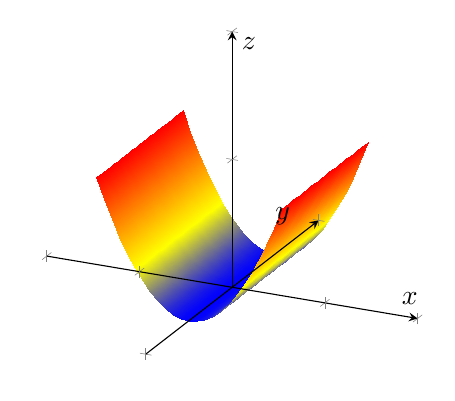
\begin{tikzpicture}
            \begin{axis}[
                width=0.7\textwidth,
                axis lines = center,
                axis on top,
                xlabel=\(x\),
                ylabel=\(y\),
                zlabel=\(z\),
                xticklabel=\empty,
                yticklabel=\empty,
                zticklabel=\empty,
                ymin=-2,
                ymax=2,
                xmin=-2,
                xmax=2,
                zmin=0,
                zmax=2]
            \addplot3[
                surf,
                domain=-1:1,
                shader = interp
            ]
            {x^2};
            \end{axis}        
        \end{tikzpicture}
    \end{figure}
\end{example}
\begin{example}
    Identify the surfaces
    \(x^2+y^2=1\)
    and \(y^2+z^2=1.\)\par \textbf{Solution: }For the first surface, there is no \(z\) dependence. So we can look at \(z\) traces and recognize them as the equations of circles with radius one in the \(xy\) plane. The graph will be a cylinder with radius \(1\) running parallel to the \(z\) axis. \par
    For the second surface, there is no \(x\) dependence. So we can look at \(x\) traces and recognize them as equations of circles with radius one in the \(yz\) plane. The graph will be a cylinder with radius one running parallel to the \(x\) axis.
\end{example}
\subsubsection{Quadric Surfaces}
A \textbf{quadric surface} is the graph of a second degree equation in terms of \(x\), \(y\), and \(z\). The general form of a quadric surface is
\[Ax^2+By^2+Cz^2+Dxy+Eyz+Fxz+Gx+Hy+Iz+J=0\]
where \(A,B,C,\dots,J\) are constants. These surfaces can be somewhat difficult to analyze, but it is doable using traces.
\begin{example}
    Use traces to describe the quadric equation
    \[\frac{x^2}{a}+\frac{y^2}{b}+\frac{z^2}{c}=1.\]\par\textbf{Solution: }First, setting \(x=k\), we get \(\frac{y^2}{b}+\frac{z^2}{c}=1-\frac{k^2}{a}\). From this, we can see that the equation is only valid when \(x\in [-\sqrt a, \sqrt a]\), and it will sketch ovals in the \(yz\) plane. \par Setting \(y=k\), we get \(\frac{x^2}{a}+\frac{z^2}{c}=1-\frac{k^2}{b}\). This is another oval, and we can see that \(y\in[-\sqrt b, \sqrt b]\).\par Finally, setting \(z=k\), we get \(\frac{x^2}{a}+\frac{y^2}{b}=1-\frac{k^2}{c}\). This is another oval, with \(z\in [-\sqrt c, \sqrt c]\).\par
    Combining all of these, we can see that the overall curve will be an egg shape centered at the origin with a radius of \(\sqrt b\) in the \(y\) direction, a radius of \(\sqrt a\) in the \(x\) direction, and a radius of \(\sqrt c\) in the \(z\) direction.
\end{example}
\begin{example}
    Use traces to describe the surface \(ax^2+by^2=cz\).\par\textbf{Solution: }First, setting \(z=k\), we get \(ax^2+by^2=ck\), which is an ellipse in the \(xy\) plane of \(x\)-radius \(\sqrt{cka^{-1}}\) and \(y\)-radius \(\sqrt{ckb^{-1}}\).\par Setting \(x=k\), we get \(by^2-cz=ak^2\), which describes a parabola in the \(yz\)-plane, opening in the \(z\) direction. \par
    Setting \(y=k\), we get \(ax^2-cz=bk^2\), which describes a parabola in the \(xz\)-plane, opening in the \(z\) direction.\par
    Overall, these three traces describe a 3D parabolic shape opening in the \(z\) direction. This type of surface is known as an \textbf{elliptic paraboloid}.
    \begin{figure}[!h]
        \centering
        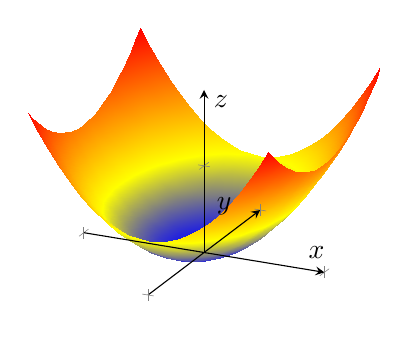
\begin{tikzpicture}
            \begin{axis}[
                width=0.5\textwidth,
                axis lines = center,
                axis on top,
                xlabel=\(x\),
                ylabel=\(y\),
                zlabel=\(z\),
                xticklabel=\empty,
                yticklabel=\empty,
                zticklabel=\empty]
                \addplot3[surf, shader=interp]{0.5 * x^2 + 0.25 * y^2};
            \end{axis}
        \end{tikzpicture}
    \end{figure}
\end{example}
\begin{example}
    Sketch the surface \(z = y^2-x^2\).\par\bf{Solution: }First, let's get the \(z\) traces by setting \(z=k\). So, \(y^2-x^2=k\), which describes a \it{hyperbola} in the \(xy\)-plane. 
    Then, the \(x\) traces tell us that \(z=y^2-k^2\), which describes a parabola opening in the \(+z\) direction in the \(yz\) plane. The \(y\) traces tell use that \(z=-x^2+k^2\) which describes a parabola opening in the \(-z\) direction in the \(xz\) plane. \par
    Together, these traces sketch a graph that looks like the one below:
    \begin{figure}[!h]
        \centering
        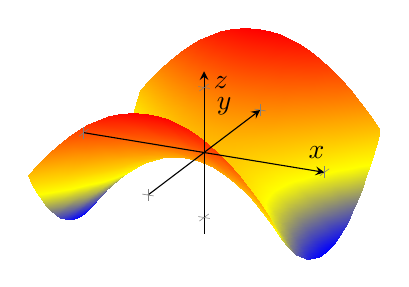
\begin{tikzpicture}
            \begin{axis}[
                width=0.5\textwidth,
                axis lines = center,
                axis on top,
                xlabel=\(x\),
                ylabel=\(y\),
                zlabel=\(z\),
                xticklabel=\empty,
                yticklabel=\empty,
                zticklabel=\empty,
                xmin =-5, xmax=5, ymin = -5, ymax=5]
                \addplot3[surf, shader=interp]{10 * y^2 - 10 * x^2};
            \end{axis}
        \end{tikzpicture}
    \end{figure}\par
    This is known as a \bf{hyperbolic paraboloid}.
\end{example}
\newpage
Some other graphs of common quadric surfaces can be seen below: {quadrics.png}
\begin{example}
    Identify and sketch the surface \(4x^2-y^2+2z^2+4=0\). \par\bf{Solution: }First, let's put the equation into standard form:
    \[-x^2+\frac{1}{4}y^2-\frac{1}{2}z^2=1.\]
    Now, we analyze the \(z\) traces to find \(\frac{1}{4}y^2-\frac{1}{2}z^2=1+k^2\), which describes a hyperbola in the \(x=k\) planes.
    The \(y\) traces tell us that \(-x^2-\frac{1}{2}z^2=1-\frac{1}{4}k^2\), which can be rearranged to say \(x^2+\frac{1}{2}z^2=\frac{1}{4}k^2-1\), which describe ovals in the \(y=k\) planes, but with a limited domain of \(|k|>2\).
    The \(x\) traces tell us that \(\frac{1}{4}y^2-\frac{1}{2}z^2=1+k^2\), which describes a hyperbola in the \(x=k\) planes.\par Together, these traces describe a \bf{hyperboloid of two sheets}, opening in the \(y\) direction.
\end{example}
\begin{example}
    Classify the quadric surface \(x^2+2z^2-6x-y+10=0\).\par\bf{Solution: }Let's first complete the square on the \(x\) terms,
    \[ [(x-3)^2-9] + 2z^2-y+10=0 \]
    And rearrange into standard form:
    \[ y-(x-3)^2-2z^2 = 1\]
    Looking at the traces, we can see:
    \begin{enumerate}
        \item \(z=k\) gives the equation \(y-(x-3)^2=1+2k^2\), describing a parabola with a positive \(y\)-intercept and facing in the \(+y\) direction.
        \item \(y=k\) gives the equation \((x-3)^2+2z^2=k-1\), describing a circle with center \((3, 0, k)\) and radius \(k\) (for \(k>1\)).
        \item \(x=k\) gives the equation \(y-2z^2=1+(k-3)^2\), describing a parabola with a positive \(y\)-intercept that opens in the \(+y\) direction.
    \end{enumerate}
    Together, these describe a hyperbola with a vertex at the coordinate \((3, 1, 0)\).
\end{example}
\subsection{Cylindrical and Spherical Coordinates}
Remember polar coordinates from single-variable calculus? It's back, with a vengaence. And now there are two of them.
\subsubsection{Cylindrical Coordinates}
Cylindrical coordinates describe points in the form \((r, \theta, z)\), where \(r\) is the distance from the origin, \(\theta\) is the angle of rotation about the \(z\) axis, and \(z\) is the height on the \(z\) axis. These are basically the same as polar coordinates, but with an added \(z\) dimension. The conversion equations are similar to polar:
\[x=r\cos\theta\quad y=r\sin\theta\quad z=z\]
and
\[r^2=x^2+y^2\quad \tan\theta = \frac{y}{x}\quad z=z\]
\begin{example}
    Convert \(P_c(2, 2\pi/3, 1)\) from cylindrical coordinates to rectangular coordinates.\par\bf{Solution: }From this, we can see that \(r=2\), \(\theta=2\pi/3\), and \(z=1\). From our conversion equations, we can determine that \(x=r\cos\theta = 2\cos(2\pi/3)=-1\) and \(y=r\sin\theta = 2\sin(2\pi/3)=\sqrt 3\). Therefore, the point is equivalent to \(P_r(-1, \sqrt 3, 1)\).
\end{example}
\begin{example}
    Find cylindrical coordinates for the point with rectangular coordinates \((3, -3, -7)\).
    \par\bf{Solution: }We can see that \(x=3\), \(y=-3\), and \(z=-7\). With our conversion formulas, \[r=\sqrt{x^2+y^2}=\sqrt{18}=3\sqrt 2\]and \[\theta = \tan^{-1}yx^{-1} = \tan^{-1}(-1)=3\pi/4+n\pi.\] Because \(x\) is positive and \(y\) is negative, \(\theta\) must be in the fourth quadrant, and we pick the solutions \(\theta=7\pi/4+2\pi n\) for any \(n\in\ZZ\). So our coordinate in cylindrical is \((3\sqrt 2, 7\pi/4+2\pi n, -7)\).
\end{example}
Cylindrical coordinates come in handy for problems that have symmetry about an axis, which we choose to be the \(z\)-axis. For example, instead of the equation \(x^2+y^2=c^2\) to describe a cylinder, we can simply use \(r=c\) to describe the same surface.
\begin{example}
    Describe the surface whose equation in cylindrical coodinates is \(z=r\).\par\bf{Solution: }For this, any coordinate \((r, \theta, r)\) is valid. In the \(z=k\) planes, the surface inscribes circles of radius \(|k|\). This suggests that our surface is a cone, which coincides with the rectangular equation \(x^2+y^2=z^2\), which we can recognize in this case as equivalent to the identity \(x^2+y^2=r^2\).
\end{example}
\begin{example}
    Find an equation in cylindrical coordinates for the ellipsoid \(4x^2+4y^2+z^2=1\)\par\bf{Solution: }First, let's rearrange the equation to the form \(4(x^2+y^2)+z^2=1\). Then, with the substitution \(r^2=x^2+y^2\), we can say that \(4r^2+z^2=1\), or \(z^2=1-4r^2\).
\end{example}
\subsubsection{Spherical Coordinates}
Spherical coordinates come in the form \(P(\rho, \theta, \phi)\). \(\rho=||\overrightarrow{OP}||\) is the distance from the origin to \(P\), \(\theta\) is the same angle as in spherical--the angle about the \(z\) axis, and \(\phi\) is the angle between the \(+z\) axis and \(P\). Note that \[\rho \geq 0, \quad 0\leq \rho\leq\pi.\]
The spherical coordinate system is handy in problems with symmetry about a point, such as cones, spheres, etc. For example, the equation \(\rho = c\) describes a sphere of radius \(C\). \(\theta=c\) describes a vertical half-plane running along the \(z\) axis. \(\phi=c\) describes a cone, stemming from the origin at an angle of \(c\) from the \(+z\) axis. 
The relationships between spherical and rectangular coordinates are shown in the picture below.
\picture{0.4\textwidth}{spherical-coordinate.png}
Namely, \begin{align*}
    r &= \rho\sin\phi \\
    x &= r\cos\theta = \rho\cos\theta\sin\phi\\
    y &= r\sin\theta = \rho \sin\theta\sin\phi\\
    z &= \rho\cos\phi
\end{align*}
And that
\[\rho^2 = x^2+y^2+z^2\]
\begin{example}
    Find the rectangular coordinates corresponding to the point \(P_s(2, \pi/4, \pi/3)\).\par\bf{Solution: }First, note that \(\rho=2\), \(\theta = \pi/4\), and \(\phi = \pi/3\). Therefore,
    \begin{align*}
        x &= \rho\cos\theta\sin\phi = 2\cdot \frac{\sqrt{2}}{2}\cdot\frac{\sqrt{3}}{2} = \frac{\sqrt 6}{2} \\
        y &= \rho\sin\theta\sin\phi = 2\cdot \frac{\sqrt 2}2\cdot \frac{\sqrt 3}2 = \frac{\sqrt 6}2 \\
        z &= \rho\cos\phi = 2\cdot \frac{1}{2} = 1
    \end{align*}
    So the point in rectangular is \(P_r(\sqrt{6}/2, \sqrt{6}/2, 1)\).
\end{example}
\begin{example}
    Find the spherical coordinates corresponding to the point \(P_r(0, 2\sqrt 3, -2)\).\par\bf{Solution: }First, we can see that \[\rho = \sqrt{x^2+y^2+z^2} = \sqrt{0^2+(2\sqrt3)^2+2^2} = 4.\]Then, we can see that \[\theta = \tan^{-1}(y/x) = \pi/4+2\pi n\](because \(\lim_{r\to\infty}\tan^{-1}r=\pi/4+2\pi n\)). Finally, we can see that \[\phi = \cos^{-1}(z/\rho)=\cos^{-1}\frac{-2}{3\sqrt 2} = \cos^{-1}\pqty{-\frac{1}{2}}=\frac{2\pi}{3}\]
    So the point in spherical coordinates is \(P_s(4, \pi/4+2\pi n, 2\pi/3)\).
\end{example}
\begin{example}
    Find an equation in spherical coordinates for the hyperboloid of two sheets with equation \(x^2-y^2-z^2=1\).\par\bf{Solution: }We can plug in our spherical coordinate version of \(x\), \(y\), and \(z\):
    \begin{align*}
        1 &= (\rho\cos\theta\sin\phi)^2-(\rho\sin\theta\sin\phi)^2-(\rho\cos\phi)^2 \\
        &= \rho^2\cos^2\theta\sin^2\phi-\rho^2\sin^2\theta\sin^2\phi-\rho^2\cos^2\phi \\
        &= \rho^2\bqty{\cos^2\theta\sin^2\phi-\sin^2\theta\sin^2\phi-\cos^2\phi} \\
        \rho &= \bqty{\sin^2\phi\pqty{\cos^2\theta-\sin^2\theta}-\cos^2\phi}^{-1/2}
    \end{align*}
\end{example}
\begin{example}
    Find a rectangular equation for the surface whose spherical equation is \(\rho = \sin\theta\sin\phi\).\par\bf{Solution: }From our conversion equations, \(y=\rho\sin\theta\sin\phi\), so \(\sin\theta\sin\phi = y/\rho\). Then,
    \begin{align*}
        \rho &= \sin\theta\sin\phi \\
        &= \frac{y}{\rho} \\
        y &= \rho ^2 \\
        &= x^2+y^2+z^2 \\
    \end{align*}
    Therefore,
    \[x^2+\pqty{y-1/2}^2+z^2=1/4\]
    Which is the equation for a sphere with center \((0, 1/2, 0)\) and radius \(1/2\).
\end{example}